\chapter{Finite-State Machines}

This thesis deals primarily with machine learning but
\cite{Silfverberg2011} presents a weighted finite-state implementation
of Hidden Markov Models. Therefore, a quick overview of finite-state
calculus is required.

\section{Weighted Finite-State Automata}

Automata can be seen as a formalization of the concept of
algorithm. They represent a restricted type of algorithm in the sense
that they can only operate on symbol strings and they only operation
they perform is to accept or reject a string. Although, this might
sound quite restrictive, it turns out that most computational problems
can be formalized as such {\it decision problems} involving only
acceptance or rejection of symbol strings.

Every automaton is associated with a {\it formal language} which is a
(possible infinite) set of finite strings from the set of all strings
of some finite alphabet. The automaton solves the decision problem of
this language, i.e. accepts exactly those strings that belong to the
language. {\it Weighted formal languages} are an extension to the
concept of formal language, where each string should be assigned a
weight. If the weights can be interpreted as probabilities, a weighted
formal language over an alphabet $\Sigma$ can be seen as a probability
distribution over the set of strings of the alphabet. However, this is
not always possible because all weights cannot be interpreted as
probabilities.

Several well know classes of algorithms exist. The most famous ones
are Turing machines which, in a sense, subsume all existing automata
\cite{?}. In this thesis I have, however, utilized another class of
automata, Finite-state machines. They are more restricted than Turing
machines or another well know class, stack automata, because they
utilize only a finite amount of memory. All real world implementations
of automata of course utilize only a finite amount of memory.

The restriction on memory limits the set of problems that finite-state
machines can solve. However, at the same time it allows for a rich
algebra which allows one to combine finite-state machines to produce
new finite-state machines.

The machine in Figure \ref{fig:np-fsm} accepts sequences of Penn
Treebank labels which correspond to singular noun phrases that can
have an adjective attribute (JJ) with an optional adverb (RB)
expressing degree.

Typically finite-state machines are represented as state transition
graphs. An example is given in Figure \ref{fig:np-fsm}. The machine
has a set of numbered {\it states} (0, 1, 2, 3 and 4) and {\it
  transitions} from one state to another. The transitions are labeled
using symbols from a finite alphabet (e.g. NN) and weights from a {\it
  weight semiring}, when the machine is weighted. The weight semiring
in this example is the {\it probability semiring} \cite{Allauzen2007}
where weights are probabilities that can be added and multiplied in
the usual fashion.

Operation starts in the designated {\it start state} (0 in Figure
\ref{fig:np-fsm}) and it has to end in a {\it final state} (2 in
Figure \ref{fig:np-fsm} marked with a double ring). A string is
accepted, if and only if there is a sequence of transitions leading
from the start state to a final state where the symbols in the
transition labels spell out the input string and the product of the
weights along the path is non-zero. For example the machine in Figure
\ref{np-fsm} accepts the string ``DT NN'' with weight 0.7 but rejects
``DT JJ'' because the string inds when the machine is in state 4 but
that is not a finite state.

There may be several or no {\it accepting paths} for a given
string. If there are several paths for some string, the machine is
called {\it ambiguous}. More generally, a machine is called {\it
  non-deterministic} if some state has several out-going transitions
with the same label. Trivially, ambiguous machines are
non-deterministic. In the case of ambiguous machines, the weight of a
string is the sum of the weights of all of its accepting paths or zero
if there are no accepting paths.

\begin{figure}
\begin{center}
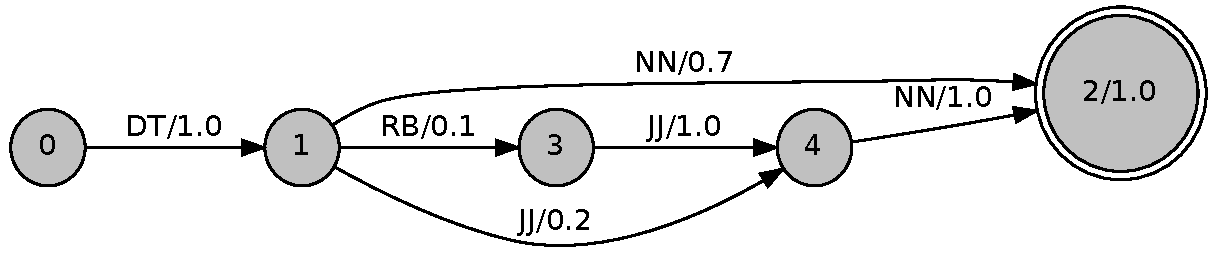
\includegraphics[scale=.7]{np}
\end{center}
\caption{A finite-state machine accepting a subset of the singular noun phrases in Penn Treebank.}\label{fig:np-fsm}
\end{figure}

\paragraph{Weighted formal languages} Formally, weighted languages are
mappings $M : \Sigma^* \rightarrow \mathbb{K}$ from the set of
arbitrary strings $\Sigma^*$ of some finite alphabet $\Sigma$ into
some {\it weight semiring} $(\mathbb{K}, \oplus, \otimes, \mathbb{0},
\mathbb{1})$ where $\mathbb{K}$ is a set of weights, $\oplus$ and
$\otimes$ are addition and product operators for weights and
$\mathbb{0} \in \mathbb{K}$ and $\mathbb{1} \in \mathbb{K}$ are the
additive and multiplicative identity.

\paragraph{Weight semirings} As mentioned above, the weight semiring
in Figure \ref{fig:np-fsm} is the probability semiring, where weights
belong to the set of non-negative reals $[0, \infty)$ and addition and
product are given by the regular real addition and product
operations. Even though probabilities reside in $[0,1]$, the addition
of probabilities can result in quantities that are larger than
$1$. Because finite-state algebra does include operations that add
probabilities, the weight set needs to include all non-negative reals.

The general weight semiring $(\mathbb{K}, \oplus, \otimes, \mathbb{0}, \mathbb{1})$ is an abstraction of the probability semiring. The set $\mathbb{K}$ is an arbitrary set but the operations $\oplus \rightarrow \mathbb{K} \times \mathbb{K} \rightarrow \mathbb{K}$ and $\oplus \rightarrow \mathbb{K} \times \mathbb{K} \rightarrow \mathbb{K}$ need to satify the following requirements \cite{Allauzen2007}
\begin{enumerate}
\item $(\mathbb{K}, \oplus, \mathbb{0})$ is a commutative and associative monoid.
\item $(\mathbb{K}, \otimes, \mathbb{1})$ is an associative monoid.
\item $\otimes$ distributes with respect to $\oplus$.
\item $\mathbb{0}$ is the annihilator of $\otimes$.
\end{enumerate}
If $\oplus$ is a group operation, the semiring is in fact a ring. Many
useful weight semirings are, however, not rings. Often the semiring
$(\mathbb{K}, \oplus, \otimes, \mathbb{0}, \mathbb{1})$ is denoted
simply as $\mathbb{K}$. Paralleling the regular sum notation $\Sigma_{i \in I} x_i$ and product notation $\prod_{i\in I} x_i$, I use the notations $\bigoplus_{i \in I} x_i$ and $\bigotimes_{i \in I} x_i$, where $I$ is a denumerable set.\footnote{Infinite sums and products are not defined in all semi rings, for example the probability semiring. In this case, it is often possible to augment the semirings with an infinity element $\infty$. This problem does not often cause problems in practice and will not be examined further.} Specifically $\oplus_{i \in \emptyset} x_i = \mathbb{0}$ and $\otimes_{i \in \emptyset} x_i = \mathbb{1}$.

Weights in the probability semiring and the addition and product operations have an intuitive interpretation but from a practical point of view the probability semiring is sub optimal. The biggest drawback is that repeated multiplication of probabilities gives rise to very small quantities and under-flow becomes a problem. Therefore, the so called {\it logarithmic semiring} is more commonly used. It can be derived by applying a logarithmic transformation $x \mapsto -\log(x)$ to the weights and operations in the probability semiring. 

In the logarithmic semiring, numerical under-flow is not a problem but
the addition operation given by $x \oplus y = -\log(\exp(-x) +
\exp(-y))$ is resource intensive. Therefore, another semiring, the
{\it tropical semiring}, is often used. The addition operation in the
tropical semiring is given by $x \oplus y = \min(x,
y)$. Computationally, this operation is light. A theoretical
motivation is given by the fact that $\min$ preserves the magnitude of
the sum although not its exact value. In practice, this is often
sufficient \cite{?}. All machines in this thesis use tropical
weights.

\paragraph{Weighted finite-state automata} Formally, a weighted
finite-state automaton of weight semiring $\mathbb{K}$ is a structure
$M = (\Sigma, Q, q_0, \rho, E)$ where
\begin{enumerate}
\item $\Sigma$ is a finite symbol set (also called an alphabet).
\item $Q$ is a finite set of states.
\item $q_0 \in Q$ is the unique start state.
\item $\rho: Q \rightarrow \mathbb{K}$ is the final weight map.
\item $T \subset Q \times (\Sigma \cup \{\epsilon\}) \times Q \times
\mathbb{K} $ is a finite set of transitions.
\end{enumerate}

The final weight map $\rho$ associates each state $q \in Q$ with a final weight. The final states of $M$ are $\{q \in Q\ | \rho(q) \ne \mathbb{0}\}$.

Each transition $x \in T$ consists of a source state $\s(x)$, an input symbol $\i(x)$, a target state $\t(x)$ and a weight $\w(x)$. The input symbol may be $\epsilon$ which denotes the empty symbol. For the single outgoing transition $x$ in state 4 in Figure \ref{fig:np-fsm}, the source state $\s(x) = 4$, the input symbol $\i(x) = {\rm "NN"}$, the target state $\t(x) = 2$ and the weight $\w(x) = 1.0$.

A sequence of transitions $x_1, ..., x_n \in T$ is a {\it path}, if
 $\s(x_1) = q_0$ and $\t(x_{k-1}) = \s(x_k)$ for all $k$. As a special case, the empty
sequence is also a path. The weight of path $p = (x_1, ..., x_n)$ is $\w_M(p) = ( \prod_{i = 1}^n \w(x_i) ) \otimes \rho(x_n)$ and the weight of the empty sequence is $\rho(q_0)$. A path $p$ is called successful when $\w_M(p) \ne \mathbb{0}$.

Each path $p = (x_1, ..., x_n)$ is associated with a unique, possibly
empty, string $s \in \Sigma^*$ such that there is a subsequence $j_i,
..., j_m$ of $1, ..., n$ for which $i(x_{j_1}), ..., i(x_{j_m}) = s$
and $i(x_{l}) = \epsilon$ whenever $l \notin \{j_1, ..., j_m\}$. If
the path $p$ is associated with the string $s$, it is called a {\it
  path of $s$}.

The set of paths of a string $s$ is denoted $P_s$ and the weight
assigned to $s$ by the automaton $M$ is $\w_M(s) = \bigoplus_{p \in
  P_s} \w_M(p)$. When $P_s = \emptyset$, $\w_M(s) = \mathbb{0}$. The
string $s$ belongs to the weighted language $L(M)$ accepted by $M$ if
$L(M)(s) = \w_M(s) \ne \mathbb{0}$.

\section{Finite-State Algebra}

Finite-state machines use only a finite fixed amount of
memory. Therefore, they cannot solve all computational problems. There
is, for example, no finite-state machine which accepts only strings of
prime number length. This can be proved using the pumping lemma of
regular language \citep{Sipser1996} which are the languages whose
decision problems finite-state automata can solve.

Although the computational power of finite-state machines is limited,
they are closed under a number of very useful operations which
correspond to set theoretical operations of the languages recognized
by the machines. The collection of these operations is called the {\it
  finite-state algebra}.

Table \ref{tab:fs-algebra} gives an overview of a number of well known
finite-state operations.

\begin{table}
\begin{center}
\begin{tabular}{lll}
Operation & Symbol & Definition \\
\hline
Union & $M_1 \oplus M_2$ & $\w_{M_1 \oplus M_2}(s) = \w_{M_1}(s) \oplus \w_{M_2}(s)$\\ 
Concatenation & $M_1 \otimes M_2$ & $\w_{M_1 \otimes M_2}(s) = \bigoplus_{s_1s_2 = s} \w_{M_1}(s_1) \otimes \w_{M_2}(s_2)$\\
Power & $M^n$ & $\w_{M^n}(s) = \bigoplus_{s_1 ... s_n = s} \w_{M}(s_1) \otimes ... \otimes \w_{M}(s_n)$\\ 
Closure & $\bigoplus_{n = 0}^\infty M^n$ &  \\
Intersection & $M_1 \cap M_2$ & $\w_{M_1 \cap M_2}(s) = \w_{M_1}(s) \otimes \w_{M_2}(s)$ \\
\end{tabular}
\caption{A selection of operators from the finite-state algebra.}\label{tab:fs-algebra}
\end{center}
\end{table}


\section{Finite-State Transducers}
Language processing frequently requires translation of one signal such
as speech or text into another signal, for example text in another
language in the case of machine translation or annotated text in the
case of part of speech tagging. These do not seem like the kinds of
processing tasks that finite-state machines can solve because, as we
saw above, finite-state machines solve decision problems.

Weighted Finite-state transducers are an extension of weighted
finite-state automata. Whereas finite-state automata simply accept or
reject a symbol sequence, finite-state transducers simultaneously
output another symbol sequence.

\begin{figure}
\begin{center}
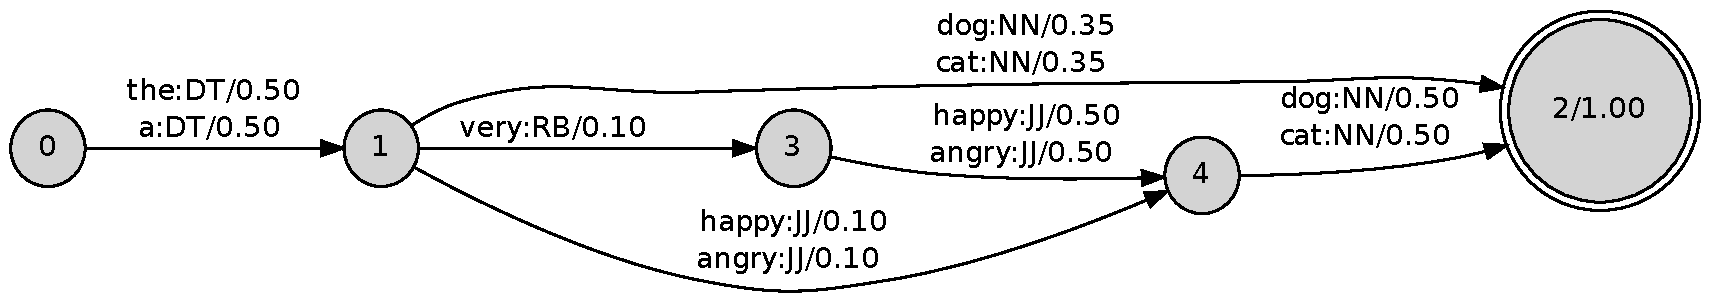
\includegraphics[scale=.5]{np_a}
\end{center}
\caption{A finite-state transducer that analyzes a subset of the singular noun phrases in Penn Treebank.}\label{fig:np-fst}
\end{figure}

Formally, a weighted finite-state transducer of weight semiring
$\mathbb{K}$ is a structure $M = (\Sigma, \Omega, Q, q_0, \rho, E)$ where
\begin{enumerate}
\item $\Sigma$ is a finite input symbol set (also called an input alphabet).
\item $\Omega$ is a finite output symbol set (also called an output alphabet).
\item $Q$ is a finite set of states.
\item $q_0 \in Q$ is the unique start state.
\item $\rho: Q \rightarrow \mathbb{K}$ is the final weight map.
\item $T \subset Q \times (\Sigma \cup \{\epsilon\}) \times (\Omega \cup \{\epsilon\}) \times Q \times
\mathbb{K} $ is a finite set of transitions.
\end{enumerate}

Transitions $e \in T$ are similar to transitions in automata but in
addition to the input symbol $\i(e)$, they also contain an output
symbol $\o(e)$. Paths of transitions are defined in the same way as
paths for automata, however, paths of transducer transitions are
associated with two strings -- an input and an output string. The
input string of path $p = (x_1, ..., x_n)$ is the string $s_i =
\i(x_1) ... \i(x_n)$ disregarding epsilons and the output string is
$s_o = \o(x_1) ... \o(x_n)$ also disregarding epsilons. Path $p$
itself is associated with the string pair $s = s_i \: s_o$. The set of
paths associated with the input string of $s$ is $\P_i(s)$ and the set
paths associated with of output string is $\P_o(s)$.

The weight of path $p$ is defined in exaclty the same way as for
automata 
$$\w_M(p) = \Big( \prod_{i = 1}^n \w(x_i) \Big) \otimes \rho(x_n).$$

A transducer $M$ can be viewed as a machine that maps input strings to
sets of output strings with weights. Equivalently, it can be seen as a
machine accepting string pairs $s = s_i \: s_o$ with some weight $\w_M(s)$. The
weight $\w_M(s)$ given to string pair $s$ by transducer $M$ is defined 
$$\w_M(s) = \bigoplus_{p \in \P_i(s) \cap \P_o(s)} \w_M(p)$$
The defition takes into account the fact that there may be several
alignments of input and output string giving the exact same string
pairs. For example, $(\epsilon\:b, a\:b)$ and $(a\:b,\epsilon\:b)$
represent the same string pair $a\:bb$.
